\chapter{急性上消化道出血}

急性上消化道出血是指食管、胃、十二指肠、胃空肠吻合术后的空肠以及胰腺、胆道的急性出血,是常见的急症,迅速确定出血部位、病因并及时处理,对预后有重要的意义。

\section{【如何确定急性上消化道出血】}

急性上消化道出血的主要临床表现是呕血与黑便,以及由于大量失血而引起的一系列全身性症状。出血量在60ml以上时则可出现柏油样黑便。一般而论,幽门以下出血时常引起黑便,而幽门以上出血则往往兼有呕血。如幽门以下部位出血量多,血液反流入胃,也可引起呕血;又如幽门以上出血量少,或出血速度缓慢,血液在胃内不引起呕吐反射,则全部血液流入肠内,自肛门排出,黑便患者可无呕血,而呕血患者则几乎均有黑便。呕出血液的性状主要决定于出血量及其在胃内停留的时间,如出血量较少或(及)血液在胃内停留时间较长,由于胃酸的作用,呕出的血液呈棕黑色咖啡渣样;反之则可呈鲜红或暗红色。上消化道出血时,粪便的颜色主要决定于出血量、出血速度及其在肠道停留的时间,其次是出血位置的高低。一般情况下,上消化道出血时,血中血红蛋白的铁与肠内硫化物结合成为硫化铁,大便呈柏油样黑色;但如出血量大,肠蠕动过快,则出现暗红色甚至鲜红色的血便。少数急性上消化道出血患者早期并无呕血或黑便,仅表现为软弱、乏力、苍白、心悸、脉搏细数、出冷汗、血压下降、休克等急性周围循环衰竭征象,须经相当时间才排出暗红色或柏油样黑便。凡患者有急性周围循环衰竭,排除急性感染、过敏、中毒及心源性等所致者,提示可能有内出血。如患者无宫外妊娠破裂、动脉瘤破裂、自发性或外伤性肝脾破裂等可能时,必须考虑急性上消化道出血,直肠指检可能较早发现尚未排出的血便。

确定为上消化道出血之前,必须排除口腔、牙龈、鼻咽等部位的出血。这些部位的出血常可在局部见到出血痕迹与损伤。呕血又须与咯血相鉴别(参见第4章)。此外,有些曾有上消化道出血史的患者,由于进食大量动物血、活性炭、某些中草药或铁剂、铋剂等而出现黑色便时,顾虑甚大,须注意区别之。

\section{【如何估计急性上消化道出血的出血量】}

急性上消化道出血症状的轻重,与失血的速度和量有关。在大出血时,患者一般有软弱、乏力、眩晕、眼花、苍白、手足厥冷、出冷汗、心悸、不安、脉搏细数,甚至昏倒等急性失血症状。少数严重失血患者早期可出现躁动、嚎叫等精神症状。综合临床表现和实验室检查,提示成人严重大出血的征象是:①患者须卧床才不头晕;②心率每分钟超过120次;③收缩压低于90mmHg或较基础血压降低25\%以上;④血红蛋白值低于70g/L。急性大出血血容量减少时,首先出现的临床表现是心搏加快,其次是血压下降,而红细胞总数与血红蛋白量下降较迟,故早期不能片面根据后两者估计失血的程度。

\section{【如何确定出血的部位与原因】}

急性上消化道出血大多数是上消化道疾病所致,少数病例可能是全身性疾病的局部出血现象,须进一步明确鉴别。前者的临床征象主要表现在上消化道局部;后者则全身症状较显著,除上消化道出血外,往往合并有其他部位出血现象。详细的病史、体检及其他检查,对出血的部位与原因有重要鉴别诊断意义。

\subsection{(一)病史}

多年慢性上腹痛病史或溃疡病病史,提示出血最大可能来自胃、十二指肠溃疡。肝炎、黄疸、血吸虫病或慢性乙醇中毒病史,有利于食管与胃底静脉曲张破裂出血的诊断。胆道蛔虫、胆石、胆道化脓性感染是胆道出血的主要原因。溃疡病出血大都发生于溃疡病活动期,故出血多见于症状发作或加重时,且多见于冬、春季节。出血时上腹痛缓解,有利于溃疡病的诊断;在右上腹剧烈绞痛缓解之后出现呕血与便血,有利于胆道出血的诊断。出血后上腹痛仍无明显缓解,常见于胃癌。食管静脉曲张破裂出血往往突然发作,血色新鲜,涌吐而出,甚至呈喷射状。伴有吞咽困难的呕血多起源于食管癌与食管溃疡。某些药物如肾上腺皮质激素、非甾体消炎药或水杨酸制剂、萝芙木制剂治疗引起的上消化道出血,往往突然发生,通常见于剂量大、疗程长的病例。

\subsection{(二)体格检查}

蜘蛛痣、肝掌、脾大、腹壁静脉怒张、腹水等病征有助于肝硬化并发食管与胃底静脉曲张破裂出血的诊断。如有左锁骨上淋巴结转移,则出血常见于胃癌。上消化道出血伴有可触及胀大的胆囊,常提示为胆道或壶腹周围癌出血。遗传性出血性毛细血管扩张症所致出血,往往可发现皮肤与口腔黏膜毛细血管扩张。

\subsection{(三)化验检查}

各项肝功能试验(包括血氨测定)有助于食管与胃底静脉曲张破裂出血的病因诊断。血细胞比容测定、红细胞计数与血红蛋白测定可估计失血的程度。出血时间、全血凝血时间、凝血酶原时间、血小板计数等出血、凝血试验及血细胞学检查,有助于出血性疾病所致的上消化道出血的病因诊断。

\subsection{(四)X线检查}

诊断未明的急性上消化道出血,吞钡检查一般均在出血停止后一段时期进行,以免诱发再次出血。细致的、特殊体位的X线检查,可能发现某些容易漏诊与罕见的病因。如采取使球后部暴露清楚的不同程度的右前斜位检查,较易发现十二指肠球后溃疡;采取头胸低位或俯卧位腹部加压、食管吞钡检查,较易发现食管裂孔疝。

\subsection{(五)急诊内镜检查}

随着内镜的普及,急性上消化道出血的病例大部分可以查明病灶,对于有明确上消化道出血的患者,在积极补充血容量、生命体征稳定的基础上,应尽快行胃镜检查以明确病因。消化性溃疡约占出血原因的50\%,其次为食管胃底曲张静脉破裂出血、各种原因引起的急性胃黏膜损伤及胃癌。虽然95\%的患者可以找到出血原因,但仍有约5\%的患者经过各种手段检查仍无无法明确出血病因。对这些出血原因不明的患者,应注意较为隐蔽或细小的病灶,如Dieulafoy病、胃肠道血管发育不良、憩室、异位胰腺等,采用各种检查手段,包括内镜、选择性腹腔动脉造影等手段尽量查明病因,为治疗提供依据。

对于出血量不大且病因未明的患者,可随访追踪观察,重复检查,直到找出病因。对出血量大且有活动性出血证据的患者,必要时可行剖腹探查加术中内镜检查以查明病因,为外科手术治疗提供依据。

胃、十二指肠镜检查目前广泛应用于上消化道出血疾病。急诊内镜检查多在出血后24~48小时举行,内镜检查不仅可观察到出血部位,还可发现新的浅表性病变与同时存在的其他病变。例如患有食管静脉曲张的病例,可能由于急性糜烂性胃炎引起出血。急诊胃十二指肠镜检查对急性糜烂性胃炎、食管贲门黏膜裂伤、应激性溃疡、吻合口溃疡、十二指肠炎等出血的诊断有决定性意义。此外还有助于出血的局部治疗,如应用局部注射、热探头、止血夹等方法止血。

\subsection{(六)其他器械检查}

床边超声检查对患者干扰甚少,有助于提示肝硬化、胆囊肿大与脾大。静脉注入放射性核素\textsuperscript{51}
铬示踪红细胞,并结合腹部扫描显像,显示出血部位的放射性浓集区,有助于肠道活动性出血灶的定位诊断。

选择性动脉造影用于诊断隐源性急性上消化道出血,有较好的评价。在这种情况下,X线钡餐检查的诊断错误率为10\%~50\%,胃镜检查有些部位观察不到,虽剖腹探查也有6\%~8\%未能找到出血部位,因此最适宜作选择性动脉造影术。原因未明的上消化道出血可作腹腔动脉造影,在静脉充盈期可使曲张的食管静脉显影。如怀疑出血部位较低,则作肠系膜上或下动脉造影,出血程度愈大,则诊断的成功率愈高,其操作快速而相当安全。禁忌证是进行性腹主动脉硬化。在胃次全切除术后患者又发生出血,此时再次手术与非手术治疗进退两难,而动脉造影有助于明确出血的部位。动脉造影能直接显示出血的病灶(肿瘤、溃疡基底),以及由于造影剂向肠腔凝聚而提示出血的部位。动脉造影发现有活动性出血时可即时进行局部填塞或滴入药物进行止血。

\section{【急性上消化道出血的原因】}

见表\ref{tab21-1}。

\begin{longtable}{c}
 \caption{急性上消化道出血疾病的分类}
 \label{tab21-1}
 \endfirsthead
 \caption[]{急性上消化道出血疾病的分类}
 \endhead
 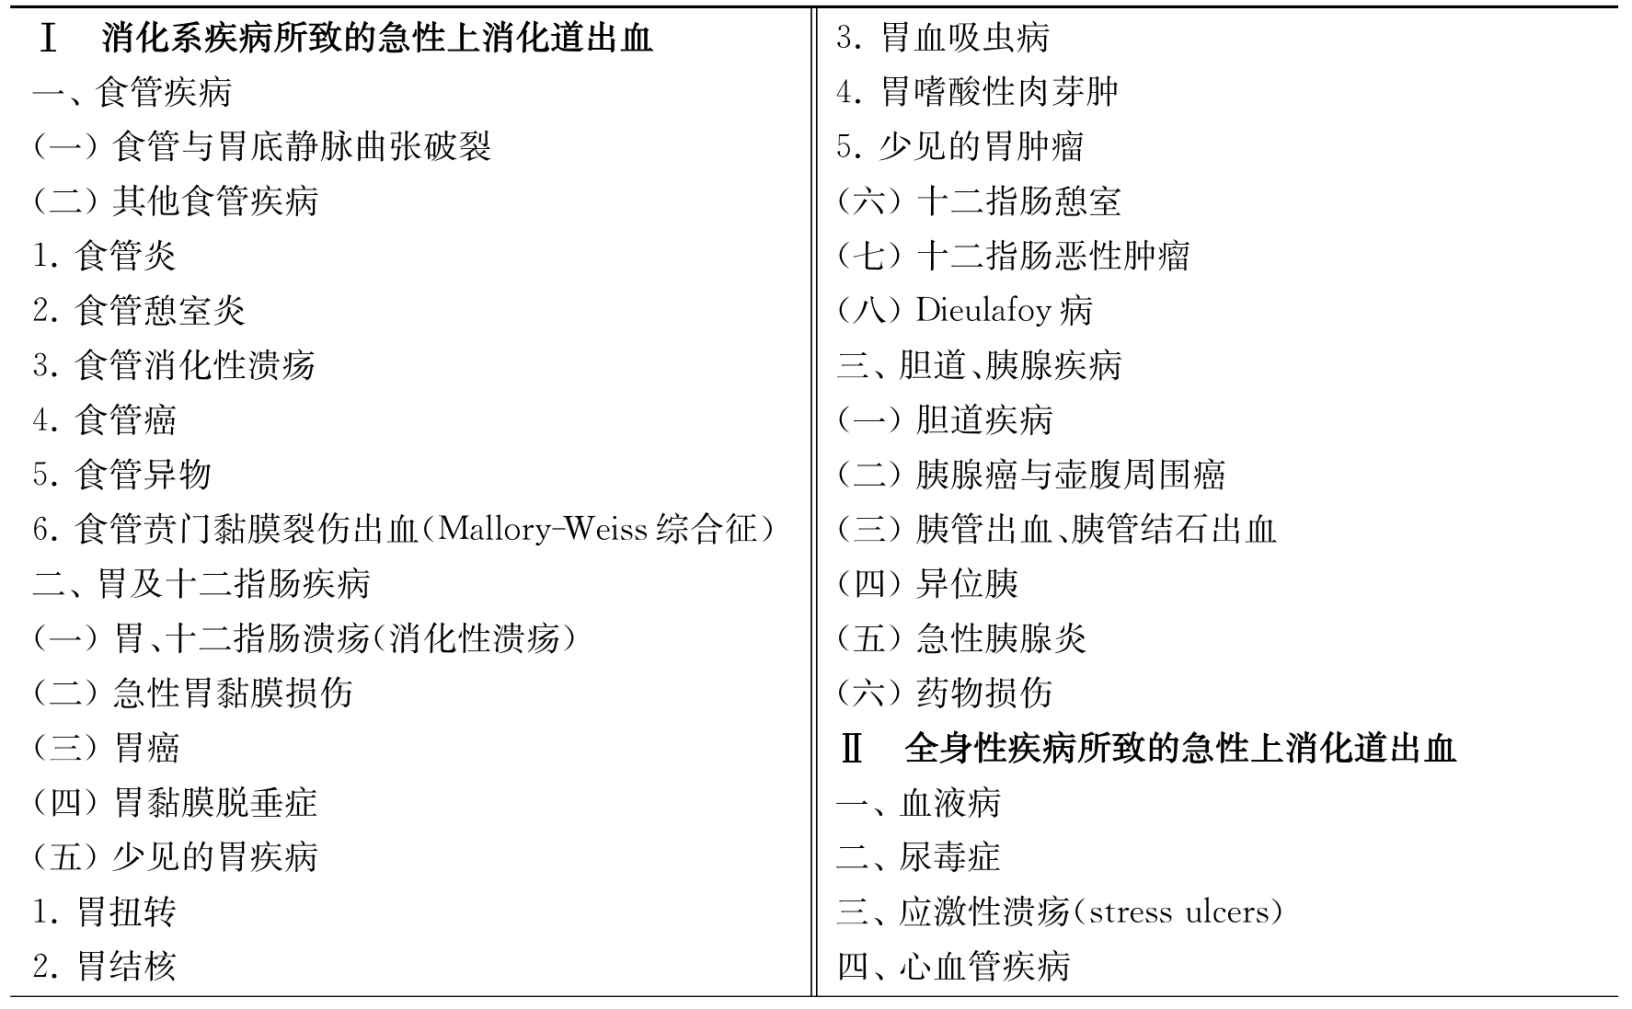
\includegraphics[width=\textwidth,height=\textheight,keepaspectratio]{./images/Image00121.jpg}\\
 
\includegraphics[width=\textwidth,height=\textheight,keepaspectratio]{./images/Image00122.jpg}
 \end{longtable}

\protect\hypertarget{text00167.html}{}{}

\section{67 消化系疾病}

\subsection{67.1 食管疾病}

\subsubsection{一、食管与胃底静脉曲张破裂}

食管与胃底静脉曲张破裂出血是肝硬化门脉高压症的严重并发症,在上消化道出血疾病中,其发病率仅次于溃疡病与出血性胃炎。临床诊断上须参考下列各项:

\paragraph{1.出血的表现}

食管与胃底静脉曲张破裂出血最突出的主诉常为呕血。呕出的血往往为鲜红色,量很多,涌吐而出,有些病例呈喷射状。患者呕血前大多有上腹部饱胀感。部分病例可呕血少而便血多,或全无呕血而仅有黑便,这是由于血液没有引起呕吐反射而按正常方向往胃肠道下行所致。有时甚至引起胃肠蠕动增强,致血液迅速从肛门排出,类似下消化道出血。一般而论,食管与胃底静脉曲张破裂出血比其他出血严重。患者有急性上消化道出血而迅速发生休克,通常多见于食管与胃底静脉曲张破裂出血或胃动脉硬化出血。

\paragraph{2.病史}

如患者过去曾有肝炎、黄疸、血吸虫病或慢性乙醇中毒历史,则对诊断肝硬化有一定的提示,但有些患者可无明确的上述病史而突然出血。另一方面,具有上述病史的患者,也可无肝硬化,仅因罹患其他上消化道疾病而致出血。

\paragraph{3.体征}

如患者有明显的肝功能损害与门脉高压病征,如巩膜黄染、蜘蛛痣、肝掌、脾大、腹壁静脉怒张、腹部移动性浊音等,则很有助于食管与胃底静脉曲张破裂出血的诊断。但须注意,轻度脾大可因大出血而暂时缩小,蜘蛛痣在大出血后也往往消失。这些情况均可使诊断困难。

肝硬化引起的食管静脉曲张破裂出血多伴有较明显的鼓肠、腹壁静脉怒张,或甚至出现腹水,而胃十二指肠溃疡出血时腹部多低平,甚少胀满。

\paragraph{4.肝功能试验}

某些肝功能检查,如血清蛋白与球蛋白比例倒置、血清蛋白电泳丙种球蛋白明显增加,均有利于肝硬化的诊断,但这些试验需时较久,对急诊病例无帮助。

\paragraph{5.急诊内镜检查}

目前应用急诊胃镜检查急性上消化道出血,在呕血停止之后即可进行,一旦发现食管静脉曲张出血,还可作硬化剂注射或静脉套扎等止血治疗。国外文献报道肝硬化与门脉高压症并发急性胃损伤出血者颇多,这时出血灶在胃而不在食管,只有经胃镜检查才能与食管静脉曲张破裂出血相鉴别。

特发性非硬化性门脉高压症甚少见,病因未明,主要表现为脾大伴脾功能亢进、食管胃底静脉曲张与反复破裂出血,而并无肝硬化的组织学改变,肝功能大多正常。

\subsubsection{二、其他食管疾病}

如上消化道出血前,患者有吞咽困难、食物反流、胸骨后或心窝部烧灼痛等症状,提示病变最大可能在食管。如临床提示有食管疾病急性出血,在病情许可时,须作胃镜检查以协助诊断。

\paragraph{(一)糜烂性食管炎}

弥漫性糜烂性食管炎或食管溃疡多由胃酸反流引起,其他引起食管溃疡的疾病尚有白塞病、克罗恩病等,真菌感染也可引起糜烂性食管炎。糜烂性食管炎可引起上消化道出血,以呕血为主,一般较慢而量少,但也有少数是大量而突然的出血,可被误诊为溃疡病出血。

表层剥脱性食管炎是少见的食管疾病,病因尚未明了。一般均有不同程度的胸骨后闷痛、呕出食物和鲜血,在反复剧烈呕吐之后突然吐出完整的管型膜状物,往往一端尚与下咽部连接,间也有完全吐出者,其构造与正常食管黏膜相同,最长可超过20cm。发病大多认为与吞咽粗糙过硬食物或鱼骨刺伤食管黏膜等有关。

\paragraph{(二)食管憩室炎}

食管憩室并发炎症或溃疡时,可发生急性出血,以呕血为主。

\paragraph{(三)食管癌}

食管癌出血往往在较晚期出现。一般为小量的持续性出血,以呕血为主,但少数病例也可发生急性大出血。

\paragraph{(四)食管异物}

食管大出血可为食管异物的严重并发症,乃由于损伤大血管所致,但大多为小量的出血。

\paragraph{(五)食管贲门黏膜撕裂}

食管贲门黏膜裂伤出血(Mallory-Weiss综合征),最多见的是由剧烈呕吐而诱发,间有因剧烈咳嗽、喷嚏等引起。凡患者在剧烈呕吐或干呕之后有呕血时,须注意此综合征的可能性,其主要表现是:①反复发作的剧烈呕吐或干呕之后出现呕血;②胃镜检查可见胃与食管交界处有黏膜裂伤,与胃、食管的纵轴相平行。但大出血时可因血液掩盖视野而胃镜检查观察不到病变,故诊断有时不易确定。国外文献报道此综合征多见于酗酒者。

\protect\hypertarget{text00168.html}{}{}

\subsection{67.2 胃及十二指肠疾病}

\subsubsection{一、胃、十二指肠溃疡(消化性溃疡)}

据我国临床资料,上消化道出血约7\%~52\%由于溃疡病所致,其中以十二指肠球部溃疡出血占多数。出血多发生于冬春两季。大多数(可达90\%)患者有长期节律性胃痛史,此点对食管静脉曲张破裂出血鉴别诊断有重要意义。反复的出血史对诊断溃疡病出血也甚有价值。如患者过去曾经X线或胃镜检查确定为溃疡病,对诊断意义尤大。

溃疡病出血常在病情恶化时发生,许多患者在饮食失调、过度精神紧张、体力劳累、受寒或感染之后突然发生出血。非甾体消炎药、肾上腺皮质激素、萝芙木制剂、磺胺类药物、抗凝剂等,均可为溃疡病出血的诱发因素。

临床症状在鉴别诊断上往往有重要的提示。多数溃疡病患者在出血前数天上腹痛加剧,对碱性药物的止痛效果不佳,出血后疼痛方见减轻。部分病例于出血前有上腹饱胀不适、食欲不振与情绪不安。呕血时多有强烈的恶心感。食管静脉曲张破裂出血则无此前驱症状,呕血时通常也无恶心感。急性胃溃疡患者有短促的胃痛史,疼痛在出血前达到最高峰,以便血兼有呕血为最常见。十二指肠溃疡以单纯便血为多见。

如上消化道出血之前有剧烈的上腹部绞痛,应注意胆道出血的可能性。胆道出血与溃疡病出血的不同点为上腹痛呈绞痛样,出血常于腹痛缓解后出现。

溃疡病出血患者过去可无胃痛史。有报道3124例溃疡病中无胃痛史而突然大出血者有48例(约占15\%)。诊断较为困难,尤其难与无肝脏病史又缺乏相应临床表现的肝硬化食管静脉曲张破裂出血相区别。急诊胃镜检查鉴别诊断价值较大。

临床上有些特殊类型的溃疡病较一般溃疡病容易发生上消化道急性大出血,如巨大溃疡、复合性溃疡、十二指肠球后溃疡、吻合口溃疡等。主要依靠钡餐X线检查或胃镜检查鉴别。

十二指肠球后溃疡:出血机会比胃、十二指肠球部溃疡高两倍多,出血量多,常反复出血,便血多于呕血,因其病变多位于后壁,易侵蚀胰十二指肠上动脉之故。

吻合口溃疡出血是胃空肠吻合术后一种严重的并发症。出血发生率较一般溃疡病为高。如胃大部分切除术后不久又发生顽固的间歇性上腹痛与上消化道出血,应考虑吻合口溃疡出血的可能性,而卓-艾综合征也须考虑。

\subsubsection{二、急性胃黏膜损伤}

急性胃黏膜损伤(糜烂性胃炎、急性胃溃疡)作为上消化道急性出血的原因近年受到重视,且不少由于药物刺激所引起。由于损伤表浅,钡餐检查难以发现,甚至在手术时也不能明显地看到。胃镜检查是最好的诊断方法。国外个别报告称急性胃损伤占上消化道出血30\%之多。急性胃黏膜损伤愈合可以较快,有时可在24小时内愈合,故胃镜检查须在出血后不久施行。

\subsubsection{三、胃 癌}

胃癌在我国常见,出血也常见,典型的呕吐物为咖啡渣样。呕血或(及)黑便可发生于任何时期,但也可为首发的症状。一般溃疡病在出血后疼痛即显著减轻或消失,而胃癌在出血后疼痛缓解往往不显著。发病在40岁以上,尤其是胃病史较短者,其出血量与贫血程度不相称时,更支持胃癌。溃疡病出血经积极治疗2~4周后,大便潜血反应转为阴性,如大便潜血持续阳性也支持胃癌的诊断。X线钡餐与胃镜检查有助于诊断(参见第81.2节)。

\subsubsection{四、胃黏膜脱垂症}

胃黏膜脱垂症是较常见的胃病,由于幽门前庭过于松弛,胃黏膜经幽门管脱入十二指肠所致。上海第二医学院附属广慈医院报告的47例中,过半数(27例)并发急性上消化道出血,多为少量的出血,以呕血为主,少数仅有便血,多同时伴有腹痛。凡急性上消化道出血患者,以往无胃病史或有不规则的胃痛史,无明显诱因与前驱症状而突然出血,或出血前几天有恶心、呕吐、腹痛加剧等前驱症状,提示胃黏膜脱垂症出血的可能性,X线钡餐或胃镜检查有助于明确诊断(参见第67.2节)。

\subsubsection{五、少见的胃疾病}

\paragraph{(一)胃扭转}

胃扭转胃扭转临床上少见,多为慢性型。患者多有节律性胃部疼痛,于餐后1~4小时出现,伴恶心、呕吐、反酸,持续2~3小时而消失。有些病例有与进食时间有关的上腹部疼痛,又可并发上消化道急性出血,这种情况和溃疡病的临床表现相似。慢性胃扭转发作时常有三大症状:剧烈的呕吐;上腹部局限性疼痛;胃管不能放入胃内。胃扭转颇常并发上消化道出血,可能由于扭转部血管与黏膜损伤所致。X线检查能明确诊断。

\paragraph{(二)胃结核}

胃结核一般为继发性,临床上很少见。患者多为30岁左右的青壮年。此病可并发出血,但急性大出血少见(参见第81.2节)。

\paragraph{(三)胃血吸虫病}

胃血吸虫病可见于血吸虫病流行区。血吸虫卵可从胃静脉逆流侵入胃壁,在黏膜与黏膜下层引起炎症与纤维组织增生。病变多位于幽门部,常引起幽门梗阻现象,或可触及上腹部包块。或因黏膜层的虫卵的机械作用和食物通过胃时的摩擦,致浅表性溃疡,并引起出血。常表现为黑便或伴有呕血。出血可严重,甚至发生休克。

胃血吸虫病并非血吸虫病的晚期现象,此时尚无肝硬化征象,且X线钡餐检查常可证明幽门梗阻和龛影,术前最易被误诊为溃疡病合并幽门梗阻或胃癌。在血吸虫病地区,患者有感染血吸虫的病史而无肝硬化的证据时,如出现上腹痛、呕吐、反酸与上消化道大出血,X线诊断为“溃疡病”,但按溃疡病积极治疗仍继续出血,应考虑胃血吸虫病出血的可能性。胃镜直视下作病理活检能确定诊断。胃次全切除术与吡喹酮治疗是有效的治疗措施。

\paragraph{(四)胃嗜酸性肉芽肿}

胃嗜酸性肉芽肿少见,临床症状、X线以及内镜下表现,均与胃癌相似,故极易误诊。有学者提到,胃溃疡、上消化道大出血、幽门梗阻、息肉样变是该病的常见并发症,主张进行胃黏膜剥离活检或深取黏膜下组织作病理学检查,以期确定诊断。

\paragraph{(五)少见的胃肿瘤}

当胃淋巴肉瘤、胃平滑肌肉瘤和胃霍奇金淋巴瘤发生破溃或溃疡形成时,均可引起急性出血,表现为黑便或呕血与黑便。这些胃肿瘤在临床上很少见,患者以壮年或中年居多,无特征性临床表现,但常有不规则的上腹痛。X线检查也难与其他胃内恶性肿瘤相区别。最可靠的诊断方法为胃内肿瘤组织或病变淋巴结的病理活检。

\subsubsection{六、十二指肠憩室}

十二指肠憩室出血一般少见,临床上与溃疡病出血不易区别,但十二指肠憩室疼痛的发生虽与饮食有关,然无一定时间性与周期性,与溃疡病不同。上消化道出血患者有类似溃疡病的症状,而X线检查无其他上消化道器质性病变发现,仅有十二指肠憩室者,应考虑十二指肠憩室出血。诊断主要依靠X线钡餐检查。憩室常位于十二指肠降段,十二指肠镜能观察到。

\subsubsection{七、十二指肠恶性肿瘤}

十二指肠恶性肿瘤的十二指肠镜诊断率甚高,一组报道显示其症状发生的几率依次为:消化道出血(58.8\%)、腹痛(55.9\%)、体重下降(52.9\%)、黄疸(32.4\%)、腹块(23.6\%)。

\subsubsection{八、Dieulafoy病}

Dieulafoy病(Dieulafoy溃疡)是由于胃肠道黏膜下层曲张的小动脉瘤破裂所致,由此可引起不同程度的出血。动脉性出血可相当严重。它最多发生在胃,少数病例可见于空肠、十二指肠与结肠。内镜直视下,出血点可呈一个帽针头大小,或为一个喷血的弯曲小血管。病变外观颇似一个部分愈合的消化性溃疡,故又名Dieulafoy溃疡。国内一组报告7例,其中6例为男性,年龄在48~76岁之间。

本病罹患大多为中、老年人。文献提到最常见于胃高位,少数见于食管、空肠、十二指肠与结肠。可发生大出血,以往多经开腹探查手术治疗。自从应用急诊内镜直视下局部注射硬化剂、无水乙醇等治疗以来,一般不需外科治疗而获得满意的止血疗效。

\protect\hypertarget{text00169.html}{}{}

\subsection{67.3 胆道、胰腺疾病}

\subsubsection{一、胆道疾病}

胆道疾病的出血比较少见,国内文献报道多因胆道感染、蛔虫及结石所引起。其他原因为肿瘤、创伤等。国内一组23例中,病因最多者为肝内化脓性感染。本病的主要临床表现是剑突下或右上腹部阵发性绞痛,疼痛缓解后出现便血或兼有呕血。如合并胆道感染则有寒战、发热。疼痛可向右肩部放射。呕出的血可混有细长条状小血块,是胆道出血所具有的特征;由于绞痛是由于血凝块堵塞胆道,引起胆道平滑肌痉挛所致,故血凝块一旦排出胆道,疼痛即缓解。约1/4~1/3患者有黄疸。胆道出血时如胆囊正常,胆囊可被血液充盈而胀大,在右上腹可触及,也是诊断胆道出血的重要体征。上述的症状常呈周期性发作与缓解,于数天或十几天之后再发。

自发性胆内瘘少见,由此引起出血者更少见。患者多为老年女性,有长期确诊的慢性胆囊炎病史,常伴有巨大结石(>2.5cm)。发作时均有一过性腹部剧痛、黄疸及发热。但出血很少影响生命体征。超声扫描提示慢性胆囊炎胆石症,须依靠开腹探查确诊。

急性胆道出血可误诊为溃疡病合并出血或胃癌合并出血。提示胆道出血的3个常有的特点是:①右上腹部或心窝处剧痛,类似胆绞痛,有时波及右侧胸部,大量呕血及便血常在腹痛减轻后出现,并出现休克症状;②可触到胀大的胆囊,往往伴有感染征象如恶寒、高热;③症状及体征消退后,一部分患者在数天或十几天内再发。B超提示胀大的胆囊。

\subsubsection{二、胰腺癌与壶腹周围癌}

胰腺癌引起出血者罕见,且发生出血时已属晚期,失去手术时机。壶腹周围癌出血比较多见,且可发生于较早期,并可出现严重的症状,但非手术的禁忌证。出血多表现为黑便,但也可伴有呕血。慢性上腹痛、营养不良、阻塞性黄疸等征象,对提示胰头癌与壶腹周围癌的诊断有重要意义。纤维十二指肠镜检查,可直接观察到Vater乳头并采取活组织作病理学诊断。B超与CT检查对胰腺癌诊断帮助甚大。

\subsubsection{三、胰管出血、胰管结石出血}

胰管出血较为罕见。病程迁延,多为上腹痛反复发作伴柏油样便,可呕吐咖啡样液体,发作时可持续数日。胰管出血的病理基础为慢性胰腺炎,胰蛋白溶解酶破坏血管壁,出血流入胰管,排入肠道。如患者既往有胰腺炎病史,伴贫血、柏油样便,便前有腹痛,反复发作,若除外胃肠道其他出血性疾病,应考虑本病。有诊断意义的检查为B超,可发现胰腺积血或积液的囊肿,也可发现胰腺搏动性包块。CT扫描可得到一个完整胰腺及其周围组织的解剖图像。内镜检查可发现出血来自胆道口壶腹。ERCP可发现胰管内血块充盈缺损,胰管中断。选择性腹腔动脉造影可发现假性动脉瘤改变。高度怀疑而出血不止的病例宜及早剖腹探查。

胰管结石是慢性胰腺炎的并发症,由结石引起的出血罕见,国内仅有个案报告。诊断方法与上述的胰管出血诊断方法相同。

\subsubsection{四、异位胰}

异位胰也称迷走胰,临床上少见。异位胰通常为单个的肿块,直径1~6cm,但也可为多发性。胃、十二指肠异位胰可在胃肠钡餐检查时发现,但多被误诊为溃疡病、良性肿瘤或胃癌。超声内镜对诊断异位胰有价值。国外文献综合589例中,异位于十二指肠30\%,胃25\%,空肠15\%,回肠3\%,梅克尔憩室6\%,此外也可异位于肠系膜、大网膜等处。异位胰有时可发生急性或慢性胰腺炎、囊样扩张、恶性或良性肿瘤而导致出血。

\subsubsection{五、急性胰腺炎}

急性重症胰腺炎可并发胃肠道黏膜出血与灶性坏死,主要发生于小肠以上的消化道,临床表现为呕血与便血。

\protect\hypertarget{text00170.html}{}{}

\subsection{67.4 药物所致的上消化道损伤}

\subsubsection{一、肾上腺皮质激素}

肾上腺皮质激素治疗加重原有的胃、十二指肠溃疡的病情,甚至引起出血、穿孔等并发症。肾上腺皮质激素性溃疡发生于长期大剂量肾上腺皮质激素的疗程中,即所谓类固醇性溃疡,与阿司匹林并用时尤易发生。疼痛无明显的节律性,常为隐袭性发展,呈所谓“无症状性”,待病变已相当严重,甚至出血或穿孔时方被发现。出血常为临床唯一的症状,且常为大量,可威胁生命。溃疡的发生无固定部位,但一般认为胃窦部多见。胃镜检查可以检出溃疡。

\subsubsection{二、非甾体消炎药}

非甾体消炎药,特别是阿司匹林(乙酰水杨酸),引起急性胃出血或胃溃疡出血者并不少见。在出血前,患者可有烧灼感、反酸与腹部不适或疼痛等症状,但也有不少患者出血前无任何消化道症状。阿司匹林对胃黏膜有刺激作用,病变局限于药物接触的胃黏膜及其周围,水杨酸制剂对出、凝血机制也有影响,故可引起相当严重的出血。

\subsubsection{三、萝芙木制剂}

萝芙木制剂,特别是利血平,不论长期的口服或注射给药,均可激发上消化道溃疡。

\subsubsection{四、抗生素}

某些抗生素,特别是口服给药时可引起胃肠反应,严重者可引起出血。曾有报告,口服青霉素由于过敏性水肿引起上消化道出血,患者可伴有急性腹痛、荨麻疹及紫癜等。曾有报告,多黏菌素引起胃肠道出血。

\subsubsection{五、其他药物}

国内外文献报道,辛可芬、组胺、咖啡因、抗癌药(如氟脲噻嘧)、甲状腺素、甲苯磺丁脲(D860)、呋喃妥因、吗啡、可待因、氨茶碱、洋地黄、抗凝剂、胰岛素、脱敏剂、白喉类毒素、雌激素,以及用于抗休克的血管收缩药如肾上腺素、去甲肾上腺素等,均可加重溃疡病或引起胃肠道黏膜损害,导致不同程度的出血。

\protect\hypertarget{text00171.html}{}{}

\section{68 全身性疾病}

\subsection{一、血液病}

各类型紫癜、白血病、再生障碍性贫血、血友病等,均可引起消化道出血。

\subsection{二、尿毒症}

尿毒症晚期可由于胃肠分泌液中氮质代谢产物含量增加,其中尿素分解后所产生的氨与铵盐,对黏膜有刺激与腐蚀作用,导致消化道黏膜糜烂与溃疡形成,并引起急性出血。血小板减少也起一定的作用。常伴有其他器官的出血现象。

\subsection{三、应激性溃疡}

应激性溃疡是急性浅表性溃疡,通常为多发性,最常发生于胃体与胃底部。在胃窦部与十二指肠通常少见。应激性溃疡大多发生于外伤后、败血症或低血压状态,往往合并黄疸、肾衰竭与呼吸功能衰竭。最常见的临床表现是无预兆的出血,但引起穿孔与梗阻者甚少。缺血与胃酸的存在是本病发病的先决条件。在这些病例中,常有胃黏膜屏障对酸类通透性增高,这种现象也可明显地参与损害的产生。溃疡可发生在重度损伤或败血症发病几小时之内,但最常见的临床病征是大出血,常发生于第2~12天之内。

应激性溃疡临床上主要见于急重症患者,因此是危险的并发症。由于大面积烧伤后发生的溃疡(Curling溃疡)曾常被认为是急性应激性溃疡的典型示例。有人将这些病例又区分为两组,最多的一组(见于14.4\%的大面积烧伤30\%以上的病例)溃疡在烧伤后最初数天内发生,为急性多发性浅表性溃疡形成,位于胃底部。这种溃疡似乎就是一般所提到的真性应激性溃疡。第二组溃疡发生较晚,常发生于烧伤的恢复期,通常位于十二指肠(见于8.9\%的烧伤病例)。在显微镜检查时,第二组溃疡显示较为慢性,很少有穿孔,有人认为是原有消化性溃疡的活动或恶化,或溃疡病素质者的溃疡形成。

由于颅内损伤、脑瘤或颅脑手术后发生的溃疡(Cushing溃疡)也曾被认为是应激性溃疡的示例。Cushing溃疡可见于食管、胃与十二指肠。这种溃疡通常深而为穿透性,偶尔整个局部胃肠壁完全溶解,引起穿孔。有人发现头部外伤时颅内压愈增高,胃液的酸度愈高。又有人发现下丘脑前核兴奋时,增加胃左动脉的血流量与胃酸分泌。研究这些患者的胃黏膜屏障对酸类的通透性,结果为正常,但胃酸分泌增加。这些观察强力揭示颅内损害所致的典型库欣溃疡,并非真正的应激性溃疡。

脑出血并发消化道出血的发生率甚高,且预后严重,由乙型脑炎引起的急性上消化道出血比其他中枢神经系统疾病所致者为多,出血与昏迷有密切关系。

应激性溃疡主要须与各种药物(如阿司匹林)或乙醇所致的糜烂性胃炎(erosive
gastritis)相区别。虽然糜烂性胃炎在临床上与病理学上和真性应激性溃疡相同,但不应列入应激性溃疡范畴。药物所致糜烂性胃炎大出血时的治疗效果,较真性应激性溃疡好得多。胃黏膜屏障的崩溃均可参与两者的发病机制。但在应激性溃疡时,胃黏膜屏障的崩溃可能由于黏膜缺血与十二指肠内容物反流入胃所致。

\subsection{四、心血管疾病}

\subsubsection{(一)心脏病}

曾有报告,急性心肌梗死合并休克、心律失常、充血性心力衰竭患者出现胃肠道出血。常为急性或死亡前出血。国外报告的370例尸检结果显示,123例(33\%)有死亡前胃肠道出血,病理解剖所见为胃、十二指肠瘀斑、糜烂或急性溃疡形成,或全肠道的广泛性黏膜出血。动脉硬化性、肺源性或心瓣膜病所致重症充血性心力衰竭的死亡病例中,常可见到广泛的肠道出血,曾有人将其命名为“死亡前出血性坏死性肠病”。

肺气肿、慢性肺源性心脏病并发胃、十二指肠溃疡的发生率颇高,其发病机制尚未完全明了。有人认为与呼吸性酸中毒所致的高碳酸血症及缺氧有关,诊断主要根据X线钡餐检查。此型溃疡的特点是隐袭性,无典型的溃疡病症状,国内报告的一组病例仅有上腹部不适感,上腹部压痛多不明显,可发生严重的大出血。

\subsubsection{(二)腹主动脉瘤}

腹主动脉瘤向肠腔穿破可引起出血,国外曾有多例腹主动脉瘤向十二指肠穿破的报告。但很少在初次发作时有血呕出。有人报告只有27\%的病例从出血至死亡时为6小时或更短。这是一个接受诊断与适当手术治疗的时机。出血可为小量或大量,常反复发作。中腹部搏动性肿块常存在,但这并非诊断必备的条件。

\subsubsection{(三)胃肠道血管瘤(hemangioma)}

可分为四种类型:①多发性静脉扩张;②海绵状血管瘤(弥漫性浸润型、息肉样型);③毛细血管瘤;④广泛性胃肠道血管瘤病(Osler-Rendu-Weber病的一种类型)。

反复的出血是胃肠道血管瘤最常见的症状。胃肠道血管瘤最常发生于小肠,但也可弥漫性分布于胃肠道或仅局限于结肠,可采用胃十二指肠镜或结肠镜观察之。X线钡餐检查有时可类似小肠的良性肿瘤,临床上有类似出血性消化性溃疡的表现。

\subsubsection{(四)遗传性出血性毛细血管扩张症}

遗传性出血性毛细血管扩张症(Osler-Rendu-Weber病)在国内曾有一组30例报告,5例有呕血。消化道出血是遗传性出血性毛细血管扩张症的严重症状,且常反复发作,有时可发生急性大出血。在颜面皮肤、口腔、鼻咽部黏膜、上肢皮肤等处发现有多发性毛细血管扩张。家族中往往有同样的病史。胃镜检查可发现高出黏膜表面、色鲜红或深红的毛细血管扩张与出血灶,并有助于除外其他原因的胃与食管出血。胃肠部分切除不能根治本病的出血,因病变为广泛性,局部治疗或偶尔雌激素治疗有效,输血对出血的治疗也有帮助。

\subsection{五、钩端螺旋体病}

钩端螺旋体病可引起胃肠道出血,但同时尚有其他器官的出血现象。

\subsection{六、结缔组织病}

肠穿孔、梗死与出血,作为系统性红斑狼疮、皮肌炎与结节性多动脉炎的胃肠道并发症,国外文献常有报告。这些并发症可出现于肾、心或肺的临床病征出现之前。

\subsection{七、弹性假黄瘤}

弹性假黄瘤是一种罕见的有遗传倾向的全身结缔组织病,主要病变为动脉中层弹性纤维变性以及内膜代偿性增厚。患者多为女性。当胃肠道血管受累时可发生上消化道大出血,尤其在妊娠期间。大多数病例的出血部位不明,不少经反复剖腹探查也未能发现。此病的特点是皮肤病变、眼底血管样条纹和视网膜损害,以及内脏广泛性血管病变。皮肤松弛,隐约可见条纹皱起,其中可见淡黄色小点状隆起,沿皮纹排列。国内文献曾报告一例并发急性上消化道出血。

\protect\hypertarget{text00172.html}{}{}

\section{参考文献}

1.洪流,等.胃嗜酸性肉芽肿的临床内镜及病理特征.中国内镜杂志,2000,6(3):29-30

2.郭春光,等.原发性十二指肠恶性肿瘤64例临床分析.中国肿瘤临床,2008,35(4):193-195

3.李峻岭,等.胰管结石引起反复上消化道大出血一例.中华内科杂志,1996,35(7):488

4.徐俊超,等.胰管出血的诊治进展.中华外科杂志,2012,50(1):77-78

5.王志益,等.表现为上消化道出血的自发性胆内瘘三例.中华内科杂志,1994,33(2):86

6.席智文,等.Mallory-Weiss综合征26例临床分析.中国内镜杂志,2004,10(11):78-79

7.陈丸,等.上消化道出血内镜检查567例分析.中华消化内镜,1999,16(3):184

8.刘俊,等.联合应用内镜注射和热凝治疗消化性溃疡出血.中华消化内镜,1999,16(1):10

9.李军婷,等.非甾体消炎药致上消化道出血的临床特征.中华消化内镜,2001,18(3):151

10.黄业斌,等.急诊内镜诊治上消化道出血183例分析.北京医学,2005,27(9):531

11.北京医学院附属第一医院内科.上胃肠道显性出血和大量出血原因的探讨.中华内科杂志,1980,19:109

12.孙光斌,等.表层剥脱性食管炎二例.中华消化内镜杂志,2006,23(6):472

13.袁二燕,等.食管-贲门黏膜撕裂综合征临床分析78例.世界华人消化杂志,2008,16(33):3796-3800

14.杨希山.Dieulafoy溃疡的诊断及治疗.中华外科杂志,1992,30:567

15.邝贺龄.Dieulafoy损害.国外医学内科学分册,1993,20:40

16.高蓓,等.慢性胃扭转12例分析.中国实用外科杂志,2002,22(12):721

17.殷凤峙.胆道疾患所致急性上消化道出血外科治疗的体会.中华外科杂志,1980,18(3):224

18.李晓勇,等.胆道出血42例的诊断和治疗.第四军医大学学报,2008,29(12):1124

19.吴在德,等.23例急性肝内胆道出血外科治疗的体会.中华外科杂志,1980,18(3):224

20.王润华.19例急性胆道出血.北京医学,1985,7:314

21.文建春.病毒性脑炎并发急性上消化道出血36例报告.北京医学,1982,4:33

22.徐文璇.脑出血与消化道出血.中华神经精神科杂志,1980,13(4):230

23.赵博旋,等.肺气肿、肺源性心脏病与溃疡病.中华内科杂志,1961,9:109

24.陆道培,等.遗传性出血性毛细血管扩张症.中华医学杂志,1973,53:543

25.陆汉明,等.弹性假黄瘤四例报告.中华内科杂志,1965,13:663

\protect\hypertarget{text00173.html}{}{}

